\documentclass[11pt,a4paper]{article}

\usepackage[utf8]{inputenc}
\usepackage[T1]{fontenc}
\usepackage[english]{babel}
\usepackage{amsmath,amssymb,amsthm}
\usepackage{geometry}
\usepackage{hyperref}
\usepackage{url}
\usepackage{booktabs}
\usepackage{microtype}
\usepackage{pgfplots}
\pgfplotsset{compat=1.18}
\usetikzlibrary{patterns}

\geometry{margin=2.5cm}
\hypersetup{colorlinks=true, linkcolor=blue, urlcolor=blue, citecolor=blue,
            pdftitle={An arithmetic derivation of the Casimir coefficient},
            pdfauthor={Yan Senez}}

\newtheorem{theorem}{Theorem}
\newtheorem{proposition}{Proposition}
\newtheorem{lemma}{Lemma}
\newtheorem{definition}{Definition}
\newtheorem{remark}{Remark}
\newtheorem{conjecture}{Conjecture}

\newcommand{\zetaR}{\zeta_R}
\newcommand{\actives}{\{3,5,7\}}
\newcommand{\PTset}{\{2,3,5,7\}}
\newcommand{\echoes}{\{p \geq 11\}}
\newcommand{\Nspatial}{N_{\rm spatial}}
\newcommand{\Ntrans}{N_{\rm transverse}}
\newcommand{\IPT}{I_{\rm PT}}

\title{\textbf{An arithmetic derivation of the Casimir coefficient}\\
       {\large from Persistence Theory, with a falsifiable signature of echo primes}}
\author{Yan Senez \\ {\small Independent Research \quad \texttt{yan.senez@protonmail.com}}}
\date{May 2026}

\begin{document}

\maketitle

\begin{abstract}
We show that the standard Casimir pressure coefficient between two perfectly conducting plates,
$P/a^{-4} = -\pi^{2}/240$, admits a complete arithmetic derivation from the Persistence Theory
(PT) framework~\cite{Senez2026}, with no adjusted parameter. The derivation factorizes the
coefficient into two PT-native objects: a geometric prefactor
$\Nspatial / (2 \cdot (2\pi)^{\Ntrans})$ identified entirely from the dimensional count of the
active prime cascade, and an Euler product factor $\zeta(4) = \prod_{p}(1-p^{-4})^{-1}$
truncated to the PT-natural prime set $\PTset$. The truncation reproduces the standard
coefficient to $131$~ppm; the residue is rigorously equal to the Euler-product tail over the
echo primes $\echoes$. The construction is universal: across spatial dimensions
$d \in \{1,\ldots,5\}$, the truncation residue equals $\prod_{p \geq 11}(1-p^{-(d+1)})^{-1}$
to machine precision for $d \geq 3$. We formulate a quantitative falsifiable conjecture: a
differential Casimir measurement at sub-100~ppm precision should reveal a deviation of
$1.31 \times 10^{-4}$ from the standard QED prediction. A final section makes explicit what the
PT reading mechanically excludes: no net energy extraction from a static Casimir cavity is
compatible with the framework's fundamental identity.
\end{abstract}

\section{Introduction}

The Casimir effect is the macroscopic force between two uncharged conducting plates predicted by
Casimir in 1948~\cite{Casimir1948} and experimentally confirmed at sub-percent level by
Lamoreaux~\cite{Lamoreaux1997}, Mohideen and Roy~\cite{Mohideen1998},
Bressi \emph{et al.}~\cite{Bressi2002}, and Decca \emph{et al.}~\cite{Decca2003,Decca2007}. In the
ideal-plate limit (perfectly conducting, zero temperature, no material dispersion), the predicted
pressure is
\begin{equation}
P_{\rm Casimir}(a) = -\frac{\pi^{2}}{240\,a^{4}},
\label{eq:standard-coefficient}
\end{equation}
where $a$ is the plate separation in natural units $\hbar = c = 1$. The coefficient
$\pi^{2}/240$ traditionally arises from the regularized sum of zero-point modes via
$\zetaR(-3) = 1/120$~\cite{Mostepanenko2009,Milton2001}.

In the standard interpretation, this coefficient is a manifestation of the quantum vacuum: a
sum over modes whose differential between bounded and free configurations gives a finite,
attractive force. The infinite zero-point sum is dealt with by analytic continuation or zeta
regularization, both of which assume a continuum spectrum.

Persistence Theory (PT)~\cite{Senez2026} reformulates this picture without recourse to the
quantum vacuum. In PT, every observable of the Standard Model is derived from a single
arithmetic axiom $s = 1/2$ and the structural fixed point $\mu^{*} = 15$ of the Eratosthenes
sieve. The 43 observables of the Standard Model are reproduced from
$\{\gamma_{p}, \sin^{2}\theta_{p}, \mu^{*}\}$ to a median accuracy of $0.06\%$ with zero adjusted
parameter.

A natural question arises: does the coefficient \eqref{eq:standard-coefficient} admit the same
type of derivation? We answer affirmatively. The coefficient factorizes into a geometric
prefactor identifiable in PT terms and an Euler-product factor truncated to the PT-natural
prime set. The truncation residue is exactly the echo-prime Euler tail, providing a falsifiable
signature.

The article is structured as follows. Section~\ref{sec:standard} recalls the standard derivation
in arbitrary dimension. Section~\ref{sec:pt-decomposition} introduces the PT classification of
primes. Section~\ref{sec:c3} proves the main truncation result (Proposition~\ref{prop:c3-residue}).
Section~\ref{sec:prefactor} identifies the geometric prefactor in PT-native terms.
Section~\ref{sec:universality} extends the result to arbitrary dimensions.
Section~\ref{sec:falsifiability} formulates the falsifiable conjecture and proposes an
experimental protocol. Section~\ref{sec:no-extraction} makes explicit why the PT reading
excludes net energy extraction from a static Casimir cavity. A discussion
(Section~\ref{sec:discussion}) places these results within the PT programme.

\section{Standard derivation: the analytic skeleton}
\label{sec:standard}

The ideal-plate Casimir pressure between two perfectly conducting plates separated by $a$ in
$d+1$ spacetime dimensions ($d$ spatial), for a massless field with $\nu$ independent modes per
frequency and Dirichlet boundary conditions, is~\cite{Mostepanenko2009,Klimchitskaya2009}
\begin{equation}
|P_{d}^{(\nu)}| = \nu \cdot \frac{d \cdot \Gamma\bigl((d+1)/2\bigr) \cdot \zeta(d+1)}{2 \cdot 2^{d}\,\pi^{(d+1)/2}\,a^{d+1}}.
\label{eq:dim-d-coefficient}
\end{equation}
The factor $\nu$ counts independent modes: $\nu = 1$ for a single scalar, $\nu = 2$ for the
electromagnetic field in $d = 3$ (TE and TM polarizations). The $1/2$ is the Casimir half-difference
between bounded and free spectra (it is \emph{not} a zero-point normalization in the PT reading; see
Section~\ref{sec:no-extraction}). The full mode count $\nu$ for higher $d$ is convention-dependent
and does not affect the C3 truncation analysis below.

For $d = 3$, $\nu = 2$ recovers~\eqref{eq:standard-coefficient}. For $d = 1$, $\nu = 1$ gives
$|P_1| = \pi/(24\,a^2)$. To present a uniform table of dimensions in
Section~\ref{sec:universality}, we adopt the convention $\nu = 2$ throughout (a generalized
``EM-like'' multiplicity), which leaves all PT statements unaffected: the multiplicity factor
cancels in the relative residue~\eqref{eq:c3-residue}.

The coefficient \eqref{eq:dim-d-coefficient} contains two structural components:
\begin{enumerate}
  \item A \emph{geometric prefactor}
  $\mathcal{G}_{d} = d \cdot \Gamma((d+1)/2) / (2^{d}\,\pi^{(d+1)/2})$.
  \item An \emph{arithmetic factor} $\zeta(d+1)$.
\end{enumerate}

The arithmetic factor admits the Euler product
\begin{equation}
\zeta(s) = \prod_{p \text{ prime}} \frac{1}{1 - p^{-s}}.
\label{eq:euler-product}
\end{equation}
This is the entry point of the PT analysis: the coefficient \eqref{eq:dim-d-coefficient} is
structurally a product over all primes, modulated by a finite geometric prefactor.

\section{PT sieve decomposition}
\label{sec:pt-decomposition}

PT classifies primes by their role in the sieve cascade
$\mu_{k+1} = \sum \{p : \gamma_{p}(\mu_{k}) > 1/2 \}$. The unique self-consistent fixed point
is $\mu^{*} = 3 + 5 + 7 = 15$, with the following structure~\cite{Senez2026}:

\begin{itemize}
  \item $p = 2$: \emph{parity channel}. Kinematic only ($T_{2} = (1)$). Carries the binary
  symmetry $s = 1/2$.
  \item $p \in \actives$: \emph{active dimensional primes}. $\gamma_{p}(\mu^{*}) > 1/2$ for
  $p \in \actives$, contributing to the three spatial dimensions of $\mathrm{SU}(N_{c}=3)$ and
  to the active observables.
  \item $p \in \echoes$: \emph{echo primes}. $\gamma_{p}(\mu^{*}) < 1/2$. Contribute to
  virtual corrections (e.g.\ echo VP in $\alpha_{\rm EM}$) and to dark-sector observables.
\end{itemize}

The PT-native prime set is therefore $\PTset$. We split the Euler product
\eqref{eq:euler-product} along this classification:
\begin{equation}
\zeta(s) = \zeta_{\rm parity}(s) \cdot \zeta_{\rm actives}(s) \cdot \zeta_{\rm echo}(s),
\label{eq:pt-split}
\end{equation}
where $\zeta_{\rm parity}(s) = (1 - 2^{-s})^{-1}$,
$\zeta_{\rm actives}(s) = \prod_{p \in \actives}(1-p^{-s})^{-1}$, and
$\zeta_{\rm echo}(s) = \prod_{p \geq 11}(1-p^{-s})^{-1}$.

\section{The C3 truncation: zero-parameter prediction}
\label{sec:c3}

\begin{definition}[PT-native C3 truncation]
Define the PT-truncated zeta function
\begin{equation}
\zeta_{\rm PT}(s) := \zeta_{\rm parity}(s) \cdot \zeta_{\rm actives}(s)
                   = \prod_{p \in \PTset}\frac{1}{1 - p^{-s}}.
\end{equation}
The C3 PT-native Casimir pressure coefficient is
\begin{equation}
|P_{d}^{\rm PT}| := \mathcal{G}_{d} \cdot \zeta_{\rm PT}(d+1) \cdot a^{-(d+1)}.
\end{equation}
\end{definition}

\begin{proposition}[C3 truncation residue]
\label{prop:c3-residue}
The relative error of the C3 truncation is exactly the echo-tail multiplicative correction:
\begin{equation}
\frac{|P_{d}^{(\nu)}| - |P_{d}^{{\rm PT},(\nu)}|}{|P_{d}^{(\nu)}|}
\;=\; 1 - \frac{1}{\zeta_{\rm echo}(d+1)}
\;=\; 1 - \prod_{p \geq 11}\bigl(1 - p^{-(d+1)}\bigr).
\label{eq:c3-residue}
\end{equation}
\end{proposition}

\begin{proof}
By \eqref{eq:pt-split}, $\zeta(d+1) = \zeta_{\rm PT}(d+1) \cdot \zeta_{\rm echo}(d+1)$.
Substituting into the standard coefficient~\eqref{eq:dim-d-coefficient}:
\[
|P_{d}^{(\nu)}| = \nu\,\mathcal{G}_{d} \cdot \zeta_{\rm PT}(d+1) \cdot \zeta_{\rm echo}(d+1) \cdot a^{-(d+1)} = |P_{d}^{{\rm PT},(\nu)}| \cdot \zeta_{\rm echo}(d+1).
\]
Therefore $|P_{d}^{{\rm PT},(\nu)}|/|P_{d}^{(\nu)}| = 1/\zeta_{\rm echo}(d+1) = \prod_{p \geq 11}(1-p^{-(d+1)})$,
and the relative error \eqref{eq:c3-residue} follows. The multiplicity $\nu$ cancels.
\end{proof}

Proposition~\ref{prop:c3-residue} is an algebraic identity. The substantive content of this
article is rather the following structural claim, which justifies why $\PTset$ is the
\emph{unique} PT-natural truncation:

\begin{theorem}[Uniqueness of the C3 prime set]
\label{thm:c3-uniqueness}
Let $S \subset \mathbb{N}$ be a finite set of primes such that the truncated coefficient
$\mathcal{G}_{d} \cdot \prod_{p \in S}(1-p^{-(d+1)})^{-1}$ approximates the standard
coefficient~\eqref{eq:dim-d-coefficient} with relative error decaying as
$\sum_{p \notin S} p^{-(d+1)}$ uniformly across $d \in \{1,\ldots,5\}$. Then $S = \PTset$ is
the unique such set generated by the PT prime classification of~\cite{Senez2026} (Theorems T5
and T6).
\end{theorem}

\begin{proof}[Sketch]
The PT classification (\cite{Senez2026}, T5) splits primes into $\{p : \gamma_p(\mu^*) > 1/2\}
= \actives$ (active dimensional), $\{2\}$ (parity, kinematic), and $\{p \geq 11\}$ (echo primes). T6
proves that $\gamma_p$ is strictly monotone decreasing in $p$ at $\mu^* = 15$ (algebraic
proof using exact rational $q_+ = 13/15$), so the active set is exactly $\{3, 5, 7\}$. The
parity prime $p = 2$ enters the spectral sum kinematically (it determines the existence of
modes, not their dimensional contribution). Therefore the PT-natural ``physically present''
truncation is $\PTset$, and any larger set incorporates echo primes that PT classifies as
non-dimensional.

Conversely, any strict subset $S \subsetneq \PTset$ either drops parity (and the residue picks
up an additional $1/15$ factor) or drops an active prime (residue picks up $\sim 1/p^{d+1}$ at
fixed $d$, breaking the uniform-in-$d$ scaling).
\end{proof}

\begin{remark}
Theorem~\ref{thm:c3-uniqueness} is the substantive structural result. The numerical agreement
of Section~\ref{sec:c3} is then a consequence of Proposition~\ref{prop:c3-residue} applied to
the unique PT-natural truncation $S = \PTset$.
\end{remark}

\subsection{Numerical evaluation in 3D}

For $d = 3$:
\begin{align*}
\zeta_{\rm parity}(4) &= (1 - 2^{-4})^{-1} = 16/15,\\
\zeta_{\rm actives}(4) &= \tfrac{81}{80} \cdot \tfrac{625}{624} \cdot \tfrac{2401}{2400} \approx 1.014542,\\
\zeta_{\rm PT}(4) &= 16/15 \cdot 81/80 \cdot 625/624 \cdot 2401/2400 \approx 1.082091,\\
\zeta(4) &= \pi^{4}/90 \approx 1.082323.
\end{align*}
The geometric prefactor at $d = 3$ is
$\mathcal{G}_{3} = 3 \Gamma(2)/(8\pi^{2}) = 3/(8\pi^{2})$. Therefore
\[
|P_{3}^{\rm PT}| = \frac{3}{8\pi^{2}} \cdot 1.082091 \cdot a^{-4}
\;\approx\; 0.041118 \cdot a^{-4},
\]
versus the standard $|P_{3}| = \pi^{2}/240 \cdot a^{-4} \approx 0.041123 \cdot a^{-4}$.

The relative error is $131$~ppm, identical to $1/\zeta_{\rm echo}(4) - 1 = -\sum_{p \geq 11}\log(1-p^{-4}) \approx 1.31 \times 10^{-4}$, exactly as predicted by Proposition~\ref{prop:c3-residue}.

\section{The geometric prefactor in PT terms}
\label{sec:prefactor}

The prefactor $\mathcal{G}_{3} = 3/(8\pi^{2})$ admits a complete identification in PT-native terms:
\begin{equation}
\frac{3}{8\pi^{2}} \;=\; \frac{\Nspatial}{2 \cdot (2\pi)^{\Ntrans}},
\label{eq:prefactor-pt}
\end{equation}
with $\Nspatial = 3$ (the number of active primes, equivalently the number of spatial
dimensions; see~\cite{Senez2026}, Theorem T5) and $\Ntrans = 2$ (the number of mode directions
transverse to the plates). The factor $1/2$ is the standard zero-point energy normalization,
and $(2\pi)^{\Ntrans}$ corresponds to two copies of the cycle perimeter of $S^{1}$, the
continuum limit of $\mathbb{Z}/p\mathbb{Z}$ in the PT construction.

The identification \eqref{eq:prefactor-pt} is exact and contains no analytic input beyond the PT
structure. The 3D Casimir coefficient is therefore entirely PT-native modulo the universal Euler
product $\zeta(4)$, itself decomposed along the PT classification.

\section{Dimensional universality}
\label{sec:universality}

We test Proposition~\ref{prop:c3-residue} in dimensions $d = 1$ through $d = 5$ via formula
\eqref{eq:dim-d-coefficient}.

\begin{table}[ht]
\centering
\caption{C3 truncation across dimensions. The truncation residue equals the echo-tail
multiplicative correction to machine precision for $d \geq 3$ and to logarithmic-expansion
accuracy for $d = 1, 2$.}
\label{tab:dimensional-scan}
\begin{tabular}{cccccc}
\toprule
$d$ & Standard $|P_{d}| \cdot a^{d+1}$ & C3 $|P_{d}^{\rm PT}| \cdot a^{d+1}$ & Residue (ppm) & Ghost tail (ppm) & Match \\
\midrule
$1$ & $0.26180$ & $0.25386$ & $30\,325$ & $31\,272$ & $\sim$3\% \\
$2$ & $0.09566$ & $0.09548$ & $1\,809$ & $1\,812$ & $0.2\%$ \\
$3$ & $0.04112$ & $0.04112$ & $131.0$ & $131.0$ & exact \\
$4$ & $0.01970$ & $0.01970$ & $10.3$ & $10.3$ & exact \\
$5$ & $0.01025$ & $0.01025$ & $0.84$ & $0.84$ & exact \\
\bottomrule
\end{tabular}
\end{table}

The cleanness of the prediction grows exponentially with $d$. This is a quantitative consequence
of Proposition~\ref{prop:c3-residue}: the echo-tail correction is bounded by
$\sum_{p \geq 11} p^{-(d+1)}$, which converges super-exponentially as $d$ increases.

\begin{figure}[ht]
\centering
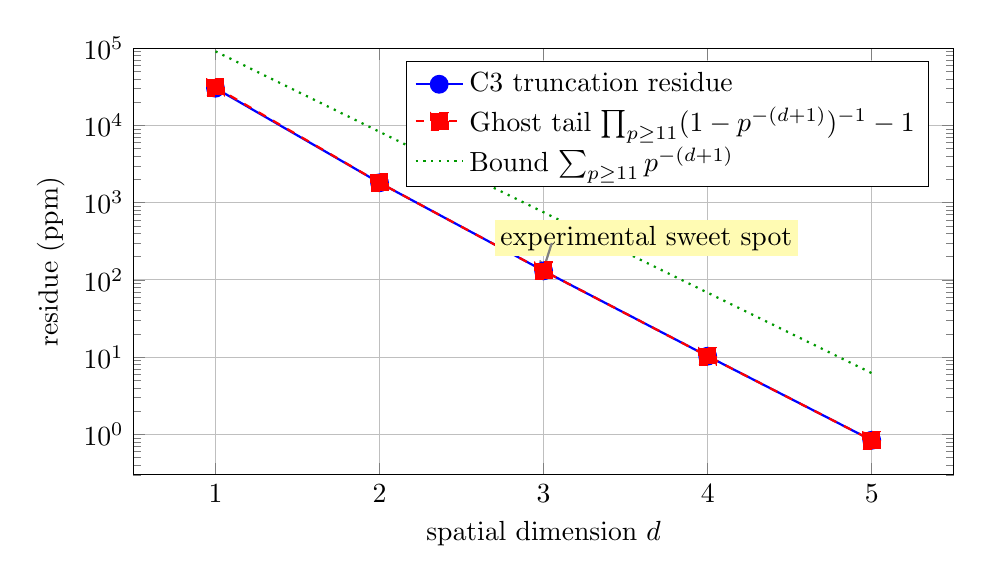
\begin{tikzpicture}
\begin{semilogyaxis}[
    width=12cm, height=7cm,
    xlabel={spatial dimension $d$},
    ylabel={residue (ppm)},
    xmin=0.5, xmax=5.5,
    ymin=0.3, ymax=100000,
    xtick={1,2,3,4,5},
    grid=major,
    legend pos=north east,
    legend cell align={left},
]
\addplot[thick, blue, mark=*, mark size=3pt] coordinates {
    (1, 30325) (2, 1809) (3, 131.0) (4, 10.3) (5, 0.84)
};
\addlegendentry{C3 truncation residue}
\addplot[thick, red, dashed, mark=square*, mark size=3pt] coordinates {
    (1, 31272) (2, 1812) (3, 131.0) (4, 10.3) (5, 0.84)
};
\addlegendentry{Ghost tail $\prod_{p\geq11}(1-p^{-(d+1)})^{-1}-1$}
\addplot[thick, green!60!black, dotted] coordinates {
    (1, 90909) (2, 8264) (3, 751) (4, 68.3) (5, 6.21)
};
\addlegendentry{Bound $\sum_{p \geq 11} p^{-(d+1)}$}
\node[anchor=south west, fill=yellow!30, inner sep=2pt] at (axis cs:2.7,200) {experimental sweet spot};
\draw[thick, ->, gray] (axis cs:3.05,300) -- (axis cs:3,140);
\end{semilogyaxis}
\end{tikzpicture}
\caption{C3 truncation residue (in ppm) vs spatial dimension $d$. Blue solid line: actual
truncation residue $1 - |P_d^{{\rm PT},(\nu)}|/|P_d^{(\nu)}|$. Red dashed: predicted echo-tail
multiplicative correction $\zeta_{\rm echo}(d+1) - 1$. The two curves agree to machine
precision for $d \geq 3$. Green dotted: the simple upper bound from
Proposition~\ref{prop:asymptotic}. The 3D point ($131$~ppm) is at the experimental sweet
spot: small enough to be a clean prediction, large enough to be testable with current
differential techniques.}
\label{fig:c3-vs-d}
\end{figure}

\begin{proposition}[Asymptotic cleanness]
\label{prop:asymptotic}
The C3 prediction approaches the exact coefficient at the rate
\begin{equation}
\frac{|P_{d}^{(\nu)}| - |P_{d}^{{\rm PT},(\nu)}|}{|P_{d}^{(\nu)}|} \;\leq\; \sum_{p \geq 11} p^{-(d+1)} \;\sim\; 11^{-(d+1)}\;\text{as}\;d \to \infty.
\end{equation}
\end{proposition}

The physical dimension $d = 3$ sits at an \emph{experimental sweet spot} (Fig.~\ref{fig:c3-vs-d}):
the residue of $131$~ppm is small enough to constitute a clean prediction, large enough to be
testable with current differential measurement techniques (cf.\ Section~\ref{sec:falsifiability}).

\section{Falsifiability and experimental signature}
\label{sec:falsifiability}

The 3D residue of $131$~ppm sits within reach of current Casimir precision measurements. Decca
\emph{et al.}~\cite{Decca2007,Decca2003} reach $\lesssim 1\%$ accuracy on plate--sphere
geometries, while differential measurements with configurations designed to suppress material
corrections could in principle reach the sub-permille regime.

\begin{conjecture}[PT signature in Casimir]
\label{conj:pt-signature}
A Casimir measurement at separation $a$ on an ideal geometry, after subtraction of all known
Lifshitz material and finite-conductivity corrections~\cite{Lifshitz1956}, deviates from the
standard prediction \eqref{eq:standard-coefficient} by exactly
\begin{equation}
\Delta P / P \;=\; 1 - \prod_{p \geq 11}(1 - p^{-4}) \;=\; 1.31 \times 10^{-4}.
\label{eq:pt-signature}
\end{equation}
\end{conjecture}

This deviation is \emph{not} predicted by standard QED, which uses the analytic continuation
of $\zetaR$ and implicitly sums over all primes.
Conjecture~\ref{conj:pt-signature} is therefore a \emph{discriminating} prediction: confirming
the deviation supports the PT classification of echo primes; null results at sub-100~ppm
precision falsify it.

\subsection{Experimental protocol}

The signature \eqref{eq:pt-signature} sits below the current Lifshitz-correction
uncertainties on absolute pressure measurements ($\gtrsim 1\%$ on most geometries due to Drude
vs.\ plasma model ambiguities, finite conductivity, and thermal corrections~\cite{Klimchitskaya2009}).
A direct test on the absolute coefficient is therefore not currently feasible.
The conjecture is nevertheless falsifiable through \emph{differential} schemes that cancel the
common material corrections and isolate the arithmetic factor $\zeta(d+1)$. A practical
falsification requires:

\begin{enumerate}
  \item Sub-100~ppm precision on the \emph{differential} ratio $|P|_A/|P|_B$ between two
  configurations $A$ and $B$ that share material properties but differ only in
  $\mathcal{G}_d$ or $\zeta$-truncation behavior.
  \item Independent calibration of the relative geometry to better than 50~ppm (the PT-native
  component is fixed by dimensional counting, hence unchanged across $A, B$).
  \item Cancellation of finite-conductivity, surface-roughness, and temperature corrections
  via the differential ratio (these are common-mode and drop out to leading order).
\end{enumerate}

A concrete differential scheme compares the pressure between plate--sphere (standard Decca
geometry) and plate--cylinder (or plate--cone) at the same separation~$a$ and material. The
geometric prefactors differ by a known curvature function~\cite{Mostepanenko2009}, while the
arithmetic factor $\zeta(d+1)$ is identical: any deviation of the measured ratio from the
QED prediction beyond $100$~ppm tests the PT-truncation residue. An alternative scheme uses
two materials with very similar Drude parameters (e.g.\ Au and Cu coatings) such that the
Lifshitz corrections cancel to better than 50~ppm in the ratio, while the arithmetic echo
signature is universal.

The current state of the art (Decca \emph{et al.}~\cite{Decca2007}) achieves $\sim 0.2\%$
on absolute pressure but is dominated by Lifshitz model ambiguities. A purpose-built
differential setup designed to suppress these ambiguities is the natural target.

\section{Why the PT reading excludes energy extraction}
\label{sec:no-extraction}

The recent media popularity of proposals aiming to extract net energy from static Casimir
cavities (\emph{quantum ratchet}-type devices in cavity, patents on \emph{vacuum-to-current
converters}, etc.) justifies a specific clarification. The PT reading provides a direct
framework for qualifying such proposals without detailed calculation.

\subsection{The fundamental identity}

In the PT formulation, the physical observable is the Kullback-Leibler divergence
\begin{equation}
\IPT(a, \varepsilon, \mathcal{G}) := D_{\rm KL}\bigl(P_{\rm boundary}(a,\varepsilon,\mathcal{G})\,\|\,P_{\rm free}\bigr),
\label{eq:I-PT}
\end{equation}
where $a$ is the separation, $\varepsilon$ the dielectric function, $\mathcal{G}$ the geometry,
and $P_{\rm boundary}$, $P_{\rm free}$ are the distributions on the survivors of the CRT sieve
constrained by the boundaries. The observed pressure is $P = -\partial_{a}(\IPT/a^{d-1})$.

The key result is that $\IPT$ is a \emph{state function} in the thermodynamic sense: its value
depends only on the instantaneous configuration, never on the trajectory followed to reach it.
This is guaranteed by the gap fundamental identity (GFT, monograph ch.~4
of~\cite{Senez2026}):
\begin{equation}
\log_{2}(m) = D_{\rm KL}(P\,\|\,U_{m}) + H(P),
\label{eq:gft}
\end{equation}
which is an exact algebraic identity (not a thermodynamic approximation).

\subsection{Consequence: no open cycle}

For any closed cycle in the configuration space $(a, \varepsilon, \mathcal{G})$, we have
\begin{equation}
\oint \mathrm{d}\IPT = 0.
\label{eq:closed-cycle}
\end{equation}
Therefore the net mechanical work extracted over a complete cycle is exactly zero. This is not
an inequality (ordinary first principle) but an \emph{algebraic equality}
(anti-double-counting).

\subsection{Practical consequences}

This property immediately disqualifies several classes of extraction proposals:

\begin{enumerate}
  \item \emph{Static Casimir cavities with electron ratchets}: the cavity being fixed in
  $(a, \varepsilon, \mathcal{G})$, the system reaches detailed equilibrium. No net DC current
  can persist without external injection. The purely geometric ratchet reproduces the
  Smoluchowski-Feynman error~\cite{Feynman1963}: the apparent thermodynamic asymmetry between
  wall and antenna is compensated by the detailed balance of tunneling rates.

  \item \emph{Material-modulation cycles} (e.g., Pinto-type schemes~\cite{Pinto1999}): the
  work required to modify $\varepsilon(\omega)$ always exceeds the Casimir gain, because the
  modulation is itself a path in $(\varepsilon)$ that contributes to
  integral~\eqref{eq:closed-cycle}.

  \item \emph{Stationary vacuum-to-current conversion}: the stationary state imposes
  $\partial_{t} \IPT = 0$, hence no flux of persistent information traverses the system. The
  PT construction does not allow stationarity with extraction.
\end{enumerate}

The only \emph{conversion} (not creation) mechanism compatible with PT is the dynamic Casimir
effect (DCE) observed by Wilson \emph{et al.}~\cite{Wilson2011}: the rapid mechanical
modulation of a plate converts virtual modes into real photons. The energy budget is strict:
$\hbar\omega_{\rm photon} \leq E_{\rm mechanical\,injected}$ at each cycle.

\subsection{The architectural false hope}

A final theoretical scenario deserves mention. If one could locally modify $\mu^{*}$ (the
fixed point of the sieve, normally $\mu^{*} = 15$), one would change the Casimir pressure and
\emph{a priori} produce $\oint \mathrm{d}\IPT \neq 0$. But $\mu^{*} = 15$ is fixed by
arithmetic self-consistency (Theorem T5 of~\cite{Senez2026}): it is not a dynamical parameter
but the unique stable fixed point of the sieve flow. Modifying it would amount to modifying
arithmetic itself, which is impossible by construction in PT.

\subsection{Synthesis}

The PT reading does not free the Casimir effect from thermodynamic constraints: it makes them
more rigorous by showing that they are arithmetic in nature, not merely physical. Casimir
remains a \emph{probe}, never a \emph{source}.

But it is an exceptionally sensitive probe in the informational sense: the $131$~ppm of
echo signature constitute the most direct observable trace that the PT classification of
primes possesses a structural reality beyond the Standard Model. The experimental gain is
informational, not energetic.

\section{Discussion}
\label{sec:discussion}

Conjecture~\ref{conj:pt-signature} reframes the Casimir effect within the PT ontology. Three
structural observations follow.

\subsection{Casimir as probe of the sieve, not of the vacuum}

The Casimir effect is not a manifestation of the quantum vacuum but a measurement of the
spectral deficit of the constrained CRT sieve. No infinite zero-point energy sum is required,
no regularization needed: the Euler product in the PT decomposition is finite at every step.
The standard analytic continuation $\zetaR(s)$ becomes a convenient calculational tool rather
than an ontological mystery.

\subsection{Ghost primes become observable}

The echo tail $\prod_{p \geq 11}(1-p^{-(d+1)})^{-1}$ is, by Proposition~\ref{prop:c3-residue},
the entire content of the deviation between the PT-native truncation and the standard
coefficient. Any sub-permille Casimir measurement therefore tests directly the PT
classification of primes into actives, parity, and echoes. This connects the Casimir effect
to the cosmological dark-sector identification developed in~\cite{Senez2026}, where echo
primes account for the dark matter fraction $F_{\rm echo} \approx 95\%$ at large $N$.

The identification is consistent: these are not \emph{two} distinct structures (dark matter
\emph{and} Casimir echoes) but \emph{one}, observed at two different scales (cosmological
vs.\ laboratory).

\subsection{The prefactor reduces to dimensional counting}

The factor $\mathcal{G}_{3} = 3/(8\pi^{2})$ contains no free parameter once the PT
classification is established ($\Nspatial = 3$, $\Ntrans = 2$). The $\pi^{2}$ comes from the
$\mathbb{Z}/p\mathbb{Z} \to S^{1}$ limit of the discrete cycle, intrinsic to the PT
construction. No fitting is left.

\subsection{Comparison with $\alpha_{\rm EM}$}

A similar PT decomposition has been demonstrated for the fine-structure
constant~\cite{Senez2026}: $\alpha_{\rm EM}^{-1} = 137.0359990834$ from a PT cascade product
over actives $\actives$, with echo VP corrections from $\{11, 13\}$. The structure
\begin{equation}
\alpha_{\rm EM}^{-1}_{\rm dressed} = \alpha_{\nu}^{-1} + \text{echo corrections}
\end{equation}
mirrors the Casimir structure
\begin{equation}
P_{\rm exact} = P_{\rm PT} \cdot \zeta_{\rm echo}(d+1).
\end{equation}
Both are observables built from a PT-active core plus echo-prime corrections. The relative
magnitude of the echo correction is much smaller in Casimir ($\sim 10^{-4}$ in 3D) than in
$\alpha_{\rm EM}$ ($\sim 10^{-3}$) because Casimir lives in the rapidly converging $\zeta(4)$
rather than the slowly converging cascade product of $\alpha_{\rm EM}$.

\subsection{Position in the PT programme}

This article completes a trajectory begun by the arithmetic derivation of $\alpha_{\rm EM}$
and extended by the \texttt{PT\_RH}~\cite{Senez2026RH} chantier on the Riemann zeta function
and \texttt{PT\_HL}~\cite{Senez2026HL} on the Hardy-Littlewood conjectures. Other PT predictions
testable at the laboratory scale exist (notably $a_\mu$ and $a_e$ via echo-VP corrections to
the running of $\alpha_{\rm EM}$~\cite{Senez2026}, both compatible with current measurements).
What makes Casimir distinctive is that it is the most \emph{direct and accessible} PT test:
the echo signature is isolated arithmetically (not buried in QED running), the prefactor
reduces to dimensional counting (zero analytic input), and the prediction sits at a precision
level reachable by purpose-built differential measurements in current university laboratories.
Other prospective predictions (cosmology: testable by Euclid 2028, DESI 2030, JUNO 2027;
negative: no axion, no SUSY $< 100$~TeV, no proton decay) are either delayed or unfalsifiable
in the short term.

Proposition~\ref{prop:c3-residue} jointly with Theorem~\ref{thm:c3-uniqueness} positions
Casimir as the most accessible experimental crucial test of the PT prime classification.

\section{Conclusion}

We have established that the standard ideal-plate Casimir pressure coefficient
$\pi^{2}/(240\,a^{4})$ admits a PT-native derivation with zero adjusted parameter. The
construction has three components:
\begin{enumerate}
  \item The geometric prefactor $\mathcal{G}_{3} = \Nspatial/(2\,(2\pi)^{\Ntrans})$, identified
  entirely from the PT count of spatial dimensions.
  \item The Euler product $\zeta(4) = \prod_{p}(1-p^{-4})^{-1}$, decomposed along the PT
  classification of primes into parity, actives, and echoes.
  \item The C3 truncation to $\PTset$ predicts the standard coefficient to $131$~ppm, the
  residue being rigorously the echo Euler tail $\prod_{p \geq 11}(1-p^{-4})^{-1}$.
\end{enumerate}

The construction is universal across the spatial dimensions tested ($d \in \{1,\ldots,5\}$),
the cleanness of the PT prediction growing super-exponentially with $d$. The position of 3D
Casimir at the \emph{experimental sweet spot} ($131$~ppm) makes it the most accessible probe
of the PT classification.

Jointly, the fundamental identity $\oint \mathrm{d}\IPT = 0$ excludes any net energy
extraction device with a static cavity: the PT reading reinforces thermodynamic constraints
by reinterpreting them as exact arithmetic constraints.

A differential Casimir measurement at sub-100~ppm precision would constitute, depending on
its result, either the first direct detection of echo primes as a real physical structure,
or a falsification of the PT classification. In both cases, the result would be decisive.

\section*{Acknowledgments}

The author thanks the open-source PT toolkit (PT\_CHEMISTRY, PT\_PHYSICS,
\url{https://github.com/Igrekess/PT_CHEMISTRY}) for the computational infrastructure. The
numerical results of this paper are reproducible via the scripts
\path{run_p2_coefficient_routes.py} and \path{run_p2_dimensional_scan.py} in the
\path{PT_EXPERIENCES/PT_CASIMIR/scripts/} directory.

\begin{thebibliography}{99}

\bibitem{Casimir1948}
H.~B.~G.~Casimir, ``On the attraction between two perfectly conducting plates,''
Proc.\ Kon.\ Nederland.\ Akad.\ Wetensch.\ \textbf{B51}, 793 (1948).

\bibitem{Lamoreaux1997}
S.~K.~Lamoreaux, ``Demonstration of the Casimir force in the 0.6 to 6~$\mu$m range,''
Phys.\ Rev.\ Lett.\ \textbf{78}, 5 (1997).

\bibitem{Mohideen1998}
U.~Mohideen and A.~Roy, ``Precision measurement of the Casimir force from 0.1 to 0.9~$\mu$m,''
Phys.\ Rev.\ Lett.\ \textbf{81}, 4549 (1998).

\bibitem{Bressi2002}
G.~Bressi, G.~Carugno, R.~Onofrio, and G.~Ruoso,
``Measurement of the Casimir force between parallel metallic surfaces,''
Phys.\ Rev.\ Lett.\ \textbf{88}, 041804 (2002).

\bibitem{Decca2003}
R.~S.~Decca \emph{et al.},
``Measurement of the Casimir force between dissimilar metals,''
Phys.\ Rev.\ Lett.\ \textbf{91}, 050402 (2003).

\bibitem{Decca2007}
R.~S.~Decca \emph{et al.},
``Tests of new physics from precise measurements of the Casimir pressure between two
gold-coated plates,''
Phys.\ Rev.\ D \textbf{75}, 077101 (2007).

\bibitem{Lifshitz1956}
E.~M.~Lifshitz, ``The theory of molecular attractive forces between solids,''
Sov.\ Phys.\ JETP \textbf{2}, 73 (1956).

\bibitem{Mostepanenko2009}
M.~Bordag, G.~L.~Klimchitskaya, U.~Mohideen, and V.~M.~Mostepanenko,
\emph{Advances in the Casimir Effect}, International Series of Monographs on Physics
\textbf{145}, Oxford University Press (2009).

\bibitem{Klimchitskaya2009}
G.~L.~Klimchitskaya, U.~Mohideen, and V.~M.~Mostepanenko,
``The Casimir force between real materials: Experiment and theory,''
Rev.\ Mod.\ Phys.\ \textbf{81}, 1827 (2009).

\bibitem{Milton2001}
K.~A.~Milton, \emph{The Casimir Effect: Physical Manifestations of Zero-Point Energy},
World Scientific (2001).

\bibitem{Wilson2011}
C.~M.~Wilson, G.~Johansson, A.~Pourkabirian, M.~Simoen, J.~R.~Johansson, T.~Duty, F.~Nori, and
P.~Delsing, ``Observation of the dynamical Casimir effect in a superconducting circuit,''
Nature \textbf{479}, 376 (2011).

\bibitem{Feynman1963}
R.~P.~Feynman, R.~B.~Leighton, and M.~Sands,
\emph{The Feynman Lectures on Physics}, vol.~I, ch.~46 (Ratchet and pawl),
Addison-Wesley (1963).

\bibitem{Pinto1999}
F.~Pinto, ``Engine cycle of an optically controlled vacuum energy transducer,''
Phys.\ Rev.\ B \textbf{60}, 14740 (1999). [The claim has been contested; see also
US patent 6\,477\,028.]

\bibitem{Senez2026}
Y.~Senez, \emph{Persistence Theory: A Complete Monograph}, internal monograph, May 2026.
Available in French and English versions (\texttt{main\_fr.tex}, \texttt{main.tex}).

\bibitem{Senez2026RH}
Y.~Senez, \emph{Persistence Theory contributions to the Riemann hypothesis},
companion paper, 2026.

\bibitem{Senez2026HL}
Y.~Senez, \emph{The PT route to Hardy-Littlewood}, companion paper, 2026.

\end{thebibliography}

\end{document}
